\chapter{¿Vivo o no vivo?}\label{ch:g1:living-or-not}

Un caracol se desliza despacio por el camino mojado. A su lado hay un
guijarro gris, igual de pequeño, igual de redondo. El caracol y el
guijarro reciben la misma lluvia --- y sin embargo uno está vivo y el
otro no. ¿Cómo lo sabemos? Esa es la primera pregunta de la \omterm{def:g1:living-or-not:living}{biología},
la ciencia de los \omterm{def:g1:living-or-not:living}{seres vivos}.

\section{Lo que hacen los seres vivos}

\begin{definition}[Ser vivo]\label{def:g1:living-or-not:living}
Un \emph{ser vivo}\index{ser vivo} es algo que está
\emph{vivo}\index{vivo}: nace, se alimenta, crece, puede tener
crías y un día muere. Los animales y las plantas son seres vivos.
La biología\index{biología} es la ciencia que los estudia.
\end{definition}

\begin{example}[El caracol y el guijarro]\label{ex:g1:living-or-not:snail}
El caracol nació de un huevo diminuto. Come hojas de lechuga. Crece
--- su concha crece con él. Puede haber caracoles bebés. Así que el
caracol es un \omterm{def:g1:living-or-not:living}{ser vivo}. El guijarro no come nada, no crece nada y
nunca tiene guijarros bebés: el guijarro no está vivo.
\end{example}


\begin{omfigure}
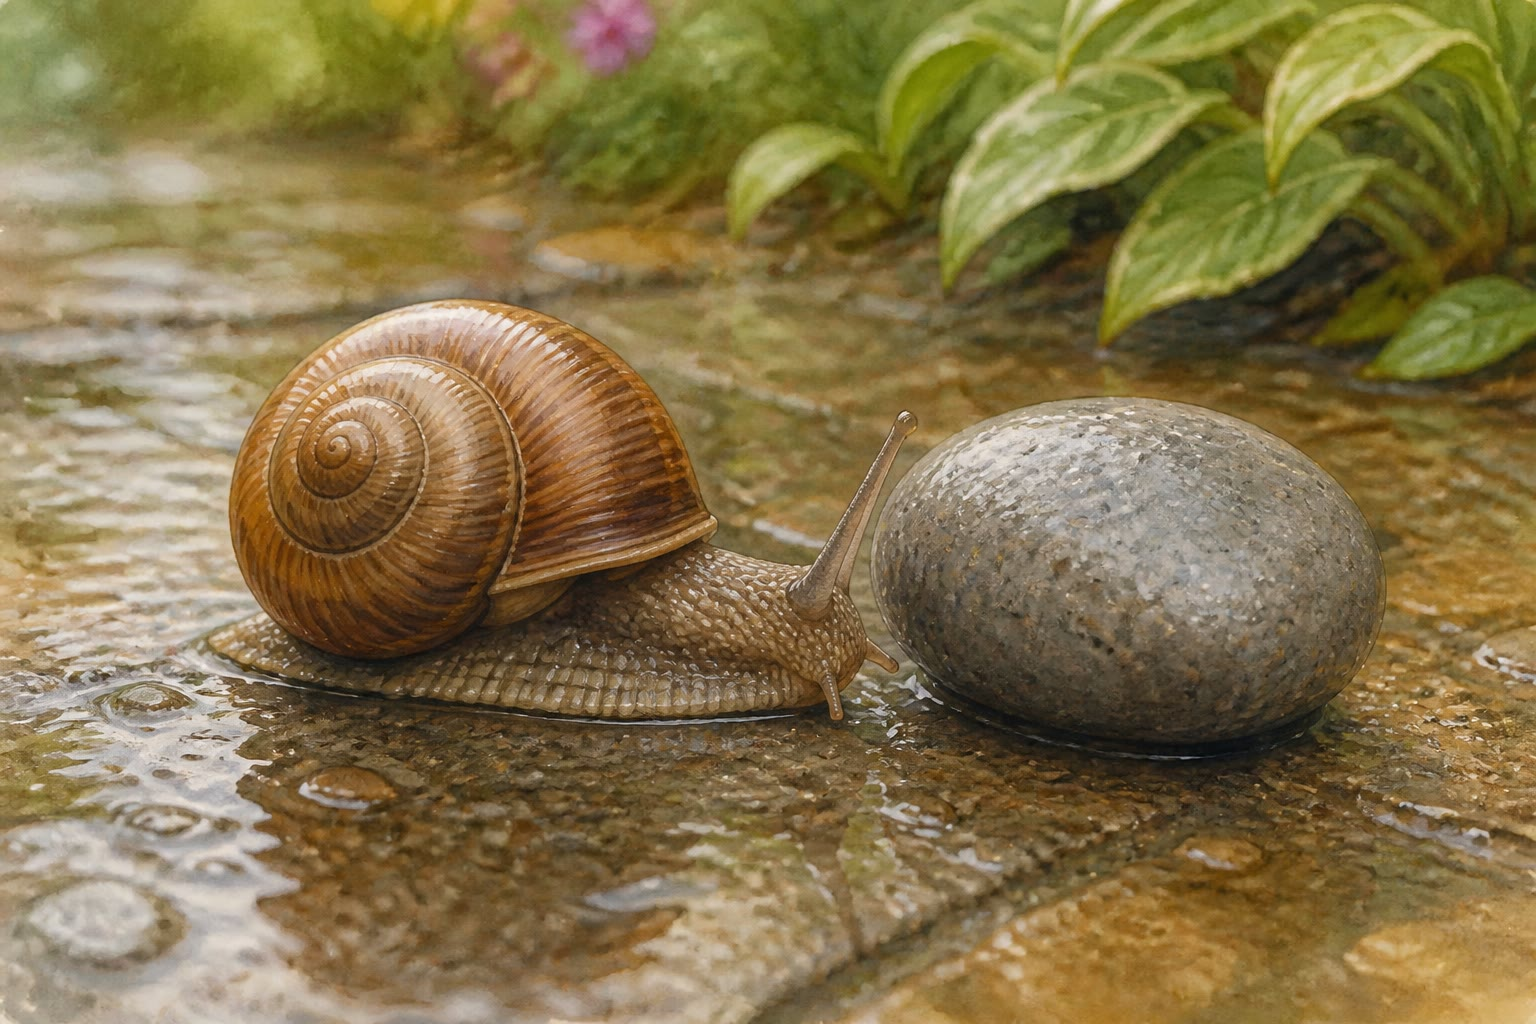
\includegraphics[width=0.62\linewidth]{images/book1/ai/g1-living-snail.jpg}

{\small Los dos vecinos del capítulo en persona: uno de ellos va
despacio hacia alguna parte, y no es el guijarro.}
\end{omfigure}

\begin{proposition}[Los signos de la vida]\label{prop:g1:living-or-not:signs}
Un \omterm{def:g1:living-or-not:living}{ser vivo} presenta estos signos:
\begin{enumerate}
  \item \emph{nace}\index{nace};
  \item \emph{se alimenta}\index{se alimenta} --- toma alimento o lo
        fabrica él mismo, como hacen las plantas con la luz;
  \item \emph{crece}\index{crece};
  \item puede tener crías --- nuevos \omterm{def:g1:living-or-not:living}{seres vivos} como él;
  \item un día \emph{muere}\index{muere}.
\end{enumerate}
Algo que no presenta ninguno de estos signos no está vivo.
\end{proposition}
\admitted

\begin{remark}[Todos los signos cuentan]\label{rem:g1:living-or-not:allsigns}
Un solo signo no basta. Un coche ``bebe'' combustible, y un carámbano
crece cuando hace frío --- pero el coche se fabricó, no nació, y el
carámbano no tiene carámbanos bebés. Para estar vivo, algo tiene que
presentar los signos de la vida \emph{juntos}: nacer, alimentarse,
crecer, hacer nuevos \omterm{def:g1:living-or-not:living}{seres vivos}, morir.
\end{remark}

\section{Vivo, no vivo, nunca vivo}

\begin{definition}[Ser inerte]\label{def:g1:living-or-not:nonliving}
Un \emph{ser inerte}\index{ser inerte} es algo que no está vivo.
Los hay de dos clases:
\begin{itemize}
  \item cosas que \emph{nunca estuvieron vivas}\index{nunca estuvo
        vivo}: un guijarro, el agua, el viento, una bicicleta;
  \item cosas que \emph{ya no están vivas}\index{ya no está vivo} o
        que \emph{proceden de} \omterm{def:g1:living-or-not:living}{seres vivos}: una hoja seca en el
        suelo, una mesa de madera, un jersey de lana.
\end{itemize}
\end{definition}

\begin{example}[La mesa de madera]\label{ex:g1:living-or-not:table}
Una mesa de madera no se alimenta y no crece: no está viva. Pero su
madera sí lo estuvo: procede de un árbol que nació de una semilla,
creció durante muchos años y fue talado. La mesa es un \omterm{def:g1:living-or-not:nonliving}{ser inerte}
--- y procede de un \omterm{def:g1:living-or-not:living}{ser vivo}.
\end{example}

\begin{example}[¿Y un robot?]\label{ex:g1:living-or-not:robot}
Un robot de juguete se mueve, hace ruidos y su luz parpadea como un
ojito. ¿Está vivo? Repasa los signos: se fabricó en una fábrica, no
nació; su pila no es un alimento que lo haga crecer; nunca tendrá
robots bebés. El robot se mueve, pero no está vivo.
\end{example}

\begin{omfigure}
\begin{tikzpicture}
  % three sorting boxes
  \draw[thick, omDef, fill=omDef!6] (0,0) rectangle (3.9,2.6);
  \draw[thick, omProp, fill=omProp!6] (4.3,0) rectangle (8.2,2.6);
  \draw[thick, omExo, fill=omExo!6] (8.6,0) rectangle (12.5,2.6);
  \node[font=\small\bfseries, omDef] at (1.95,2.25) {vivo};
  \node[font=\small\bfseries, omProp] at (6.25,2.25) {estuvo vivo};
  \node[font=\small\bfseries, omExo] at (10.55,2.25) {nunca vivo};
  \node[font=\small, align=center, text width=3.6cm] at (1.95,1.1)
    {un caracol\\ una margarita\\ ¡tú!};
  \node[font=\small, align=center, text width=3.6cm] at (6.25,1.1)
    {una hoja seca\\ una cuchara de madera\\ una pluma en el camino};
  \node[font=\small, align=center, text width=3.6cm] at (10.55,1.1)
    {un guijarro\\ un charco\\ una canica};
\end{tikzpicture}

{\small Tres cajas para clasificar el mundo: vivo, ya no vivo,
nunca vivo.}
\end{omfigure}

\begin{method}[¿Cómo decidir: vivo o no vivo?]\label{met:g1:living-or-not:decide}
Hazte las preguntas de la vida, una a una:
\begin{enumerate}
  \item ¿Nació? ¿Se alimenta? ¿Crece?
  \item ¿Puede tener crías? ¿Morirá algún día?
  \item Si las respuestas son sí: está vivo.
  \item Si las respuestas son no, hazte una pregunta más:
        ¿\emph{procede de} algo vivo, como la madera de un árbol?
\end{enumerate}
\end{method}

\begin{remark}[Las semillas parecen dormidas]\label{rem:g1:living-or-not:seed}
Una semilla seca de judía, dentro de su sobre, parece tan quieta como
un guijarro. Pero ponla sobre algodón mojado y, en unos días, asoma
una raicita: la semilla estaba viva todo el tiempo, esperando. Los
\omterm{def:g1:living-or-not:living}{seres vivos} lentos y silenciosos se confunden fácilmente con los
inertes --- las preguntas de la vida nos ayudan a mirar más de cerca.
\end{remark}

\section{Ejercicios}

\begin{exercise}[$\star$]\label{exo:g1:living-or-not:1}
Di los cinco signos de la vida. ¿Cuáles de ellos puedes ver hacer hoy
a un gatito?
\end{exercise}

\begin{exercise}[$\star$]\label{exo:g1:living-or-not:2}
¿Vivo o no vivo? (a) una mariposa; (b) una bicicleta; (c) una
margarita; (d) una nube.
\end{exercise}

\begin{exercise}[$\star$]\label{exo:g1:living-or-not:3}
Una hoja seca está en el camino. ¿Está viva ahora? ¿Lo estuvo alguna
vez? ¿De dónde viene?
\end{exercise}

\begin{exercise}[$\star$]\label{exo:g1:living-or-not:4}
Tomás dice: ``El río está vivo --- ¡mira, se mueve y hace ruido!''
Usa las preguntas del \cref{met:g1:living-or-not:decide} para
responderle con cariño.
\end{exercise}

\begin{exercise}[$\star$]\label{exo:g1:living-or-not:5}
Clasifica en las tres cajas de la figura --- vivo, estuvo vivo, nunca
vivo: una araña, un calcetín de lana, una gota de lluvia, una manzana
en el árbol, una piña caída.
\end{exercise}

\begin{exercise}[$\star$]\label{exo:g1:living-or-not:6}
La llama de una vela ``come'' la cera, se hace más alta y muere
cuando soplas. ¿Es la llama un \omterm{def:g1:living-or-not:living}{ser vivo}? ¿Qué pregunta de la vida
dice que no?
\end{exercise}

\begin{exercise}[$\star$]\label{exo:g1:living-or-not:7}
Nombra dos cosas de tu habitación que procedan de \omterm{def:g1:living-or-not:living}{seres vivos}, como
la mesa de madera del \cref{ex:g1:living-or-not:table}. Di de qué
\omterm{def:g1:living-or-not:living}{ser vivo} procede cada una.
\end{exercise}

\begin{exercise}[$\star$]\label{exo:g1:living-or-not:8}
Pruébalo: pon una judía seca sobre algodón mojado cerca de una
ventana, y un guijarro sobre otro trozo de algodón mojado al lado.
Míralos cada día durante una semana. ¿Cuál cambia? ¿Qué demuestra eso?
\end{exercise}

\begin{exercise}[$\star\star$]\label{exo:g1:living-or-not:9}
Un robot de juguete y un caracol se mueven los dos por el suelo. Da
dos preguntas de la vida en las que sus respuestas sean distintas.
\end{exercise}

\begin{exercise}[$\star\star$]\label{exo:g1:living-or-not:10}
Las setas no corren como los animales y no son verdes como la mayoría
de las plantas. Con los signos de la
\cref{prop:g1:living-or-not:signs}, explica por qué una seta es de
todas formas un \omterm{def:g1:living-or-not:living}{ser vivo}.
\end{exercise}
